\section {Background}

\subsection{Tommy John Surgery}

The surgery was first performed by Dr. Frank Jobe in 1974 on Tommy John due to irreversible damage done to the ulnar collateral ligament (UCL) in his pitching arm. As such UCL reconstruction surgery has become known as Tommy John surgery. The surgery replaces the damaged UCL in the pitching arm elbow of with a tendon from another body part. Originally the replacement tendon was taken from the forearm, however more recently doctors have favoured harvesting from the hamstring.

The degree to which requiring TJS affects a pitchers ability to return to play varies. However, several studies have reported between 67\% to 83\% of Major League Baseball (MLB) pitchers who underwent TJS returned to play at the same level \cite{Erickson2014} \cite{Cain2010} \cite{Makhni2014}. While the prospects for return are promising, it has been reported that it can take upwards of 16 months to return \cite{Makhni2014}. This is concerning to both the player and their team, especially if the are under a large contract.

It is widely believed by athletes and coaches that performance can actually improveme as a result of TJS \cite{Conte2015}. However, increases in performance after TJS can be related to strength gains during rehabilitation or mechanical improvements \cite{Cain2010}. The improvements may not even be real as the lower stats prior to the injury could be a result of impaired performance due to smaller injuries leading up to a full UCL tear. \cite{Makhni2014}. As such, there are no data to support prophylactic UCL reconstruction to improve performance or prevent injuries \cite{Erickson2014}

\subsection{Ulnar Collateral Ligament}

The UCL is a thick triangular ligament where each side of the triangle is a separate ligament (Figure \ref{fig:ucl_sketch}). The entire structure is located in the middle of the elbow toward the body. Of the three sub-ligaments, the anterior oblique ligament is the most important in terms of stress and forces. The anterior oblique ligament is commonly what is referred to as the UCL, as such we will also simply refer to the UCL.

\begin{figure}[ht]
    \centering
        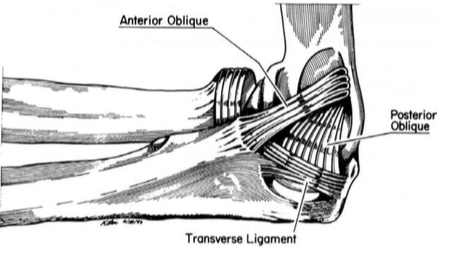
\includegraphics[width=0.45\textwidth]{ucl_sketch}
    \caption{Three sub ligaments make up the UCL. \cite{Safran2005}}
    \label{fig:ucl_sketch}
\end{figure}

\begin{figure}[hb]
    \centering
        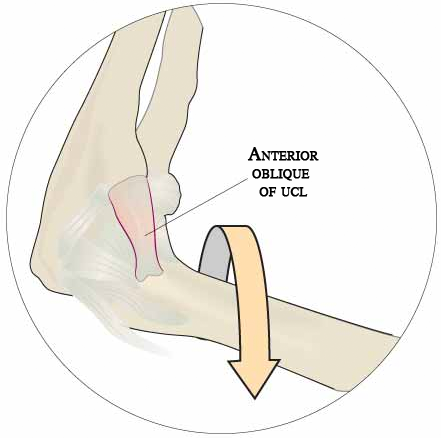
\includegraphics[width=0.3\textwidth]{ucl_torque}
    \caption{As arm rotates high valgus stress is generated on the UCL. \cite{NYTucl}}
    \label{fig:ucl_torque}
\end{figure}

Pitching generates high valgus and extension forces across the elbow \ref{fig:ucl_torque} during late cocking and acceleration phases. Stress is highest on the UCL when the elbow is flexed 90\degree and the shoulder is rotated away from the body \ref{fig:arm_pos} \cite{Fleisig2015}. At this point the anterior bundle of UCL is the primary restraint against valgus stress at the elbow. During this motion it is thought the vagus load approaches the maximum tensile strength of the UCL. It is therefore possible that a pitchers throwing elbow gradually leads to failure as a result of repeatedly being exposed to near-failure stresses \cite{Cain2010}

\begin{figure}[h]
    \centering
        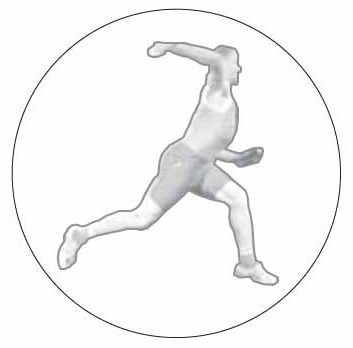
\includegraphics[width=0.3\textwidth]{arm_pos}
    \caption{Greatest valgus stress occurs during the late cocking phase of the pitchers throw. \cite{NYTucl}}
    \label{fig:arm_pos}
\end{figure}

Biomechanical studies have shown that moments of force on the shoulder and elbow as well as valgus torque are higher for fastballs than other pitches \cite{Keller2016}. This would suggest that pitchers that throw more fastballs could have an increased risk to UCL damage and thus increase chance of requiring TJS.

Given such a high prevlance of of TJS in professional baseball it is frustrating to all parties involved that diagnosing an UCL injury is difficult and likely not made until well after damage is done. One study suggested that diagnosis of UCL damage not made until an average of 6.4 months after symptoms began \cite{Cain2010}. One reason is can be so difficult to diagnose is that partial tearing of the UCL is likely indistinguishable from normal elbow laxity on examination. However, a player questionnaire reported that 96\% of players acknolwedged pain during the late cocking and acceleration phases of throwing \cite{Cain2010}. As such proper diagnosis may require a more qualitative analysis by team doctors with players.

\subsection{Risk Factors}

Many risk factors have been speculated including mechanics, pitch type, fatigue, overuse, velocity, and medical issues \cite{Keller2016} \cite{Fleisig2015}. However, proper investigation of the issue has been difficult. It has only been recently that the prevelance of TJS has been investigated and risk factors are only beginning to be uncovered \cite{Conte2015}. The ability to determine risk factors is also limited by studies being retrospective in nature. This limits the ability of researchers to determine changes in factors such as mechanics.

\subsection{Identifying Players at Risk}

\subsubsection{Common Statistics}

Several studies have made an attempt to find a relationship between declines in common pitcher statistics and the player requiring TJS. Comparing the pitchers statistics after returning from surgery hows shown a performance decrease, however the significance varies widely \cite{Makhni2014}. Also, several case-controlled studies failed to find a statistical difference between controls and injury pitchers \cite{Jiang2014} \cite{Erickson2014}.

It has been argued that common statistics like earned runs average (ERA), batting average against (BAA), and walks plus hits divided by innings pitched (WHIP) are not the best measures to consider when trying to investigate risk factors or predictors for TJS \cite{Gray2014}. This is due to the fact that these statistics are also affected by the ballpark the game is played in, the skill of the rest of the defense, luck, and several other factors. Factors more specific a pitchers performance would include fielding-independent pitching (FIP), pitch velocity, pitch type, movement, and other variables tracked for each pitch thrown by a pitcher.

\subsubsection{Pitch Specific Measures}

Every stadium in MLB has been equipped with the Sportvision PITCHf/X system. This system consists of 2 cameras located in the stands above home plate and first base. The purpose of these cameras is to track the flight of every pitch thrown and determine its position, velocity and acceleration \cite{Fast2010}. The system is paired with an MLB employee that records further information abouth the pitch such as strike, top and bottom of strike zone, etc.

Studies focusing directly on PITCHf/X data has also been varied. This could be largely due to the fact the classification algorithm used by the PITCHf/X system is constantly being tweaked so comparing data over multiple years can be counfounded by variation inherent in the system \cite{Fast2010}. In an attempt to overcome this several groups including the website http://brooksbaseball.net reviews all PITCHf/X data and manually reclassifies errors confirmed by their research.

While there can be a lot of noise present in the PITCHf/X data it is still useful to analyze. A study of 38 pitchers who had undergone TJS reported a small but significant decrease in the velocity of fastballs post injury \cite{Jiang2014}. However, a more recent study a larger sample size (83) failed to find a significant decrease in fastball velocity \cite{Keller2016}. Both studies were case-controlled and reported no significant difference in velocity between groups. However, it was reported that pitchers requiring TJS pitched a significantly higher percentage (7\%) of fastballs than controls. This suggests that the number of fastballs thrown is a risk factor but not the velocity of the pitch itself. \cite{Keller2016} Another study found decreases were observered in percentage of fastballs thrown and pitches in strike zone up to 2 years after surgery \cite{Makhni2014}. This may be related to changes in mechanics post surgery.

\subsubsection{Injury History}
A difficult set of factors to investigate in regards to players being at risk of UCL injury is previous injuries to the throwing arm, specifically the elbow. Difficulties are related to the available data on player injuries. Traditionally teams have preferred to hold exact details regarding their player's injuries, therefore data reported publically may not be accurate. However, in more recent years more data surrounding player injuries has become available and is making it easier to investigate.

One study looked at players being placed on the disabled list (DL), a public record of players removed from the teams active roster due to injury. The authors reported before surgery 74\% of players were placed on DL because of an injury to their throwing arm and of these 58\% were elbow related. After surgery 57\% of players were placed on DL because of an injury to their throwing arm, of which 26\% were an elbow injury \cite{Makhni2014}. This study was case-controlled and no significant difference was found between groups for total number of times placed on the DL for injuries related to the throwing arm. However, a higher number of of players requiring TJS went to DL specifically for elbow related injuries \cite{Makhni2014}.